\section{Diagrama de Casos de Uso}

\begin{figure}[h]
\begin{center}
	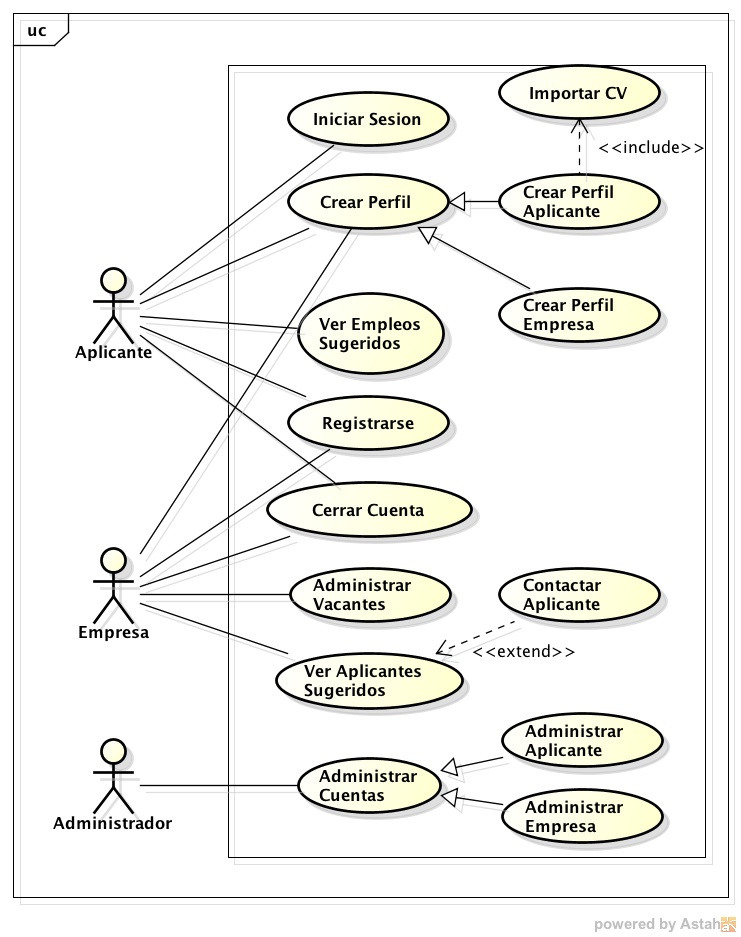
\includegraphics[scale=0.71]{./resources/UserCaseDiagram.png}
	\caption{Diagrama de Casos Usos}
	\label{fig:User: casediagram}
\end{center}
\end{figure}

\newpage
%\subsection{Modelo de comportamiento}
%A continuación se presentan las trayectorias correspondientes a los casos de uso del sistema "Buscador de Ofertas Laboral %TI"


\subsection{Caso de Uso 1: Registrarse}
\textbf{DESCRIPCIÓN COMPLETA}
\newline 

En este caso de uso el actor proporcionara la información básica para la apertura de una cuenta, la cual le permitirá proporcionar los datos necesarios al sistema para la vinculación Empleado-Empleador.\newline \newline


\textbf{ATRIBUTOS IMPORTANTES:}

\begin{table}[h]			
        \begin{center}			
        \begin{tabular}{|l|p{11cm}|} \hline
        
        			
Nombre del caso de uso	&	Registrarse.	\\ \hline
Versión	&	1	\\ \hline
Actor(es)	&	Aplicante, Empresa.	\\ \hline
Propósito	&	Crear una cuenta para comenzar a utilizar el sistema.	\\ \hline
Resumen	&	Los actores proporcionarán un correo electronico y una contraseña para que el sistema generé una cuenta.	\\ \hline
Entradas	&	o         Nombre.	\\ 
	&	o         Tipo de usuario	\\
	&	o         Correo electronico.	\\
	&	o         Contraseña.	\\ \hline
Salidas	&	Mensaje de confirmación de su registro.	\\ \hline
Precondiciones	&	No estar registrado en el sistema.	\\ \hline
Post condiciones	&	No aplica.	\\ \hline
Autor	&	David Hernández Muñoz.	\\ \hline
Tipo	&	Primario.	\\ \hline



\end{tabular}			
        \caption	{	CU Registrar	}
        \label	{tabla	1	}
        \end{center}			
\end{table}			


\textbf{TRAYECTORIA PRINCIPAL}
\begin{enumerate}
\item	\textbf{User:  }Ingresa a la página del sistema.
\item	\textbf{System: }Muestra la pantalla principal del sistema.
\item	\textbf{User:  }Da click la sección de “Registrarse”.
\item	\textbf{System: }Muestra pantalla con el formulario correspondiente al registro.
\item	\textbf{User:  }Seleccionar que tipo de usuario se registrará (Aplicante/Empresa).
\item	\textbf{User:  }Ingresa en el formulario un nombre, correo electrónico y contraseña.
\item	\textbf{User:  }Presiona el boton de “Registrar”.
\item	\textbf{System: }Muestra mensaje de registro exitoso.
\item	\textbf{System: }Redirecciona a la pantalla de inicio de sesión.
\end{enumerate}
----Fin de la trayectoria.



\newpage
\subsection{Caso de Uso 	2	: Iniciar Sesión	}
		\textbf{DESCRIPCIÓN COMPLETA}	
		\newline 	
		Para que el usuario pueda gestionar su información y realizar posibles contactos, debe iniciar sesión. 	\newline \newline
		\textbf{ATRIBUTOS IMPORTANTES:}	
\begin{table}[h]			
        \begin{center}			
\begin{tabular}{|l|p{11cm}|} \hline			
Nombre del caso de uso	&	Iniciar Sessión.	\\ \hline
Versión	&	1	\\ \hline
Actor(es)	&	Aplicante.	\\ \hline
Propósito	&	Iniciar sesión en el sistema para hacer uso de los servicios proporcionados.	\\ \hline
Resumen	&	El usuario se identificará ingresando nombre de usuario y contraseña.	\\ \hline
Entradas	&	Nombre de Usuario y Contraseña.	\\ \hline
				
			
Salidas	&	Llave de sesión, mensaje de éxito al iniciar sesión y redirección a la pantalla de inicio.	\\ \hline
Precondiciones	&	Estar registrado en el sistema.	\\ \hline
Post condiciones	&	No aplica.	\\ \hline
Autor	&	David Hernández Muñoz	\\ \hline
Tipo	&	Primario.	\\ \hline
\end{tabular}			
        \caption	{	CU Iniciar Sesión	}
        \label	{tabla	2	}
        \end{center}			
\end{table}			

\textbf{TRAYECTORIA PRINCIPAL}			
\begin{enumerate}			
\item \textbf{	User: 	}	Ingresa a la pagina del sistema.
\item \textbf{	User: 	}	Da click la sección de “Iniciar  sesión”.
\item \textbf{	System: 	}	Muestra pantalla con el formulario correspondiente al inicio de sesión.
\item \textbf{	User: 	}	Ingresa: nombre de usuario y contraseña.
\item \textbf{	User: 	}	Presiona el boton de “iniciar Sesión”.
\item \textbf{	System: 	}	Muestra la pantalla principal del sistema.
			
			
			
\end{enumerate}			
----Fin de la trayectoria.			





\newpage			
\subsection{Caso de Uso 	3	: Crear Perfil	}
		\textbf{DESCRIPCIÓN COMPLETA}	
		\newline 	
		Despues de que el usuario concluya su registro en el sistema, procedera a crear su perfil el cual consiste en proporcionar al sistema información relevante para el Empleado y el Empleador.	\newline \newline
		\textbf{ATRIBUTOS IMPORTANTES:}	


\begin{table}[h]			
        \begin{center}			
\begin{tabular}{|l|p{11cm}|} \hline			
Nombre del caso de uso	&	Crear Perfil.	\\ \hline
Versión	&	1	\\ \hline
Actor(es)	&	Aplicante, Empresa.	\\ \hline
Propósito	&	Registrar los datos del actor según sea el caso para su procesamiento en el sistema.	\\ \hline
Resumen	&	El usuario ingresará información clave según sus caracteristicas, para que el sistema pueda organizarlo y relacionarlo según sea el caso: con los contratantes o clientes potenciales. 	\\ \hline
Entradas	&	Aplicante:\\
&o Nombre.\\
&o Edad.\\
&o Dirección.\\
&o Profesión.\\
&o Habilidades o aptitudes\\
&o Curriculum Vitae (PDF).\\
&o Contacto\\
& Empresa:\\
&o Nombre.\\
&o Razón Social.\\
&o Dirección.\\
&o Telefono.\\
&o Contacto. \\
&o Descripció de actividades.	\\		\hline
Salidas	&	Mensaje: Registro exitoso	\\ \hline
Precondiciones	&	1. Estar registrado.\\
& 2. Haber iniciado sesión.
	\\ \hline
Post condiciones	&	No aplica.	\\ \hline
Autor	&	David Hernández Muñoz	\\ \hline
Tipo	&	Primario.	\\ \hline
\end{tabular}			
        \caption	{	CU Crear Perfil	}
        \label	{tabla	2	}
        \end{center}			
\end{table}			

\textbf{TRAYECTORIA PRINCIPAL}			
\begin{enumerate}			
\item \textbf{	User: 	}	Seguimeinto del Caso de Uso “Iniciar  sesión”.
\item \textbf{	User: 	}	Da click en la sección de “Crear Perfil”.
\item \textbf{	System: 	}	Muestra pantalla con el formulario correspondiente al registro.
\item \textbf{	User: 	}	Ingresa los datos del formulario.
\item \textbf{	User: 	}	Presiona el boton de “Crear Perfil”.
\item \textbf{	System: 	}	Muestra mensaje:  “Perfil creado con éxito”.
\item \textbf{	System: 	}	Muestra la pantalla principal del sistema.
			
			
\end{enumerate}			
----Fin de la trayectoria.			



\newpage			
\subsection{Caso de Uso 	4	: Ver Empleos Sugeridos	}
		\textbf{DESCRIPCIÓN COMPLETA}	
		\newline 	
		En esta parte el Aplicante podra visualizar una lista que el sistema generará según las características y conveniencias del mismo. De esta forma el sistema será un facilitador para la busqueda del empleo.	\newline \newline
		\textbf{ATRIBUTOS IMPORTANTES:}	

\begin{table}[h]			
        \begin{center}			
\begin{tabular}{|l|p{11cm}|} \hline			
Nombre del caso de uso	&	Ver Empleos Sugeridos.	\\ \hline
Versión	&	1	\\ \hline
Actor(es)	&	Aplicante.	\\ \hline
Propósito	&	Que el aplicante pueda ver los empleos según sus actitudes, aptitudes y conveniencias.	\\ \hline
Resumen	&	Cuando el aplicante seleccione la sección de “Ver Empleos Sugeridos” se le desplegará en pantalla los empleos con los que el sistema lo allá relacionado.	\\ \hline
Entradas	&	Llave de sesión	\\ \hline
			
			
			
			
Salidas	&	Listado de empresas con las que tenga relación.	\\ \hline
Precondiciones	&	1. Estar registrado en el sistema.\\
&2. Haber iniciado sesión.
	\\ \hline
Post condiciones	&		\\ \hline
Autor	&	David Hernández Muñoz	\\ \hline
Tipo	&	Primario.	\\ \hline
\end{tabular}			
        \caption	{	CU Ver Empleos Sugeridos	}
        \label	{tabla	4	}
        \end{center}			
\end{table}			


\textbf{TRAYECTORIA PRINCIPAL}			
\begin{enumerate}			
\item \textbf{	User: 	}	Seguimeinto del Caso de Uso “Iniciar  sesión”.
\item \textbf{	User: 	}	Da click en la sección de “Empleos Sugeridos”.
\item \textbf{	System: 	}	Muestra una lista de los empleos especificos para el usuario.
			
\end{enumerate}			
----Fin de la trayectoria.			




\newpage			
\subsection{Caso de Uso 	5	: Cerrar Cuenta	}
		\textbf{DESCRIPCIÓN COMPLETA}	
		\newline 	
		Cuando el Aplicante o Empresa decidan precindir de los servicios ofrecidos, bastará con ingresar en la sección “Cerrar Cuenta”, en la cual se le informa que sus datos serán borrados del sistema y que la vinculación Empleado-Empleador ofrecida por medio de nuestro sistema se perderá.	
\newline	\newline	\textbf{ATRIBUTOS IMPORTANTES:}	

\begin{table}[h]			
        \begin{center}			
\begin{tabular}{|l|p{11cm}|} \hline			
Nombre del caso de uso	&	Cerrar Cuenta.	\\ \hline
Versión	&	1	\\ \hline
Actor(es)	&	Empresa, Aplicante.	\\ \hline
Propósito	&	Que el actor se de de baja en el sistema y desvincular sus datos con el posible solicitante o empleador. 	\\ \hline
Resumen	&	El actor derminará que la información que proporciono al sistema no se encuentre disponible para su vinculación y visualización. Los datos seran borrados del sistema de almacenamiento.	\\ \hline
Entradas	&	Llave de sesión	\\ \hline
			
			
			
			
Salidas	&	Mensaje de confirmación de “Cuenta Cerrada”.	\\ \hline
Precondiciones	&	1. Estar registrado.\\
& 2. Haber iniciado sesión.\\ \hline
Post condiciones	&	El usuario no prodrá ingresar al sistema.	\\ \hline
Autor	&	David Hernández Muñoz	\\ \hline
Tipo	&	Primario.	\\ \hline
\end{tabular}			
        \caption	{	CU Cerrar Cuenta	}
        \label	{tabla	5	}
        \end{center}			
\end{table}			

\textbf{TRAYECTORIA PRINCIPAL}			
\begin{enumerate}			
\item \textbf{	User: 	}	Seguimeinto del Caso de Uso “Iniciar  sesión”.
\item \textbf{	System: 	}	Muestra pantalla con el formulario correspondiente para cerrar una cuenta.
\item \textbf{	User: 	}	Ingresa contraseña
\item \textbf{	User: 	}	Ingresa la justificación del cierre de la cuenta.
\item \textbf{	User: 	}	Presiona el boton  “Cerrar cuenta”.
\item \textbf{	System: 	}	Muestra mensaje: “Los datos y vinculaciones serán borrados.¿Desea Continuar? ”.
\item \textbf{	User: 	}	Presiona el boton  “Si”.
\item \textbf{	System: 	}	Muestra mensaje: “Cuenta cerrada satisfactoriamente”.
\item \textbf{	System: 	}	Redirecciona a la pagina princilal.
\end{enumerate}			
----Fin de la trayectoria.			




\newpage			
\subsection{Caso de Uso 	6	: Registro de empresa	}
		\textbf{DESCRIPCIÓN COMPLETA}	
		\newline 	
		En esta parte podremos revisar las distintos tipos de vista que el usuario podrá ver al hacer la página 	
\newline	\newline	\textbf{ATRIBUTOS IMPORTANTES:}	

\begin{table}[h]			
        \begin{center}			
\begin{tabular}{|l|p{11cm}|} \hline			
Nombre del caso de uso	&	Crear empresa	\\ \hline
Versión	&	1	\\ \hline
Actor(es)	&	Empresa, Administrador	\\ \hline
Propósito	&	Crear un nuevo perfil de una empresa para registrar vacantes	\\ \hline
Resumen	&	Cada que una nueva empresa quiera postular vacantes en el sitio web deberá crear un perfil de la empresa especificando datos solicitados la empresa deberá ser validada por un administrador para evitar fraudes	\\ \hline
Entradas	&	o Nombre	\\ 
&		o Dirección	\\
&		o Teléfono	\\
&		o Rubro	\\
&		o Nombre y teléfono del representante legal	\\\hline
Salidas	&	Mensaje de solicitud en tramite	\\ \hline
Precondiciones	&	Que la empresa que solicita no esté ya previamente registrada	\\ \hline
Post condiciones	&	Ninguna	\\ \hline
Autor	&	Gómez Ponce Alberto Xavier	\\ \hline
Tipo	&	Primario	\\ \hline
\end{tabular}			
        \caption	{	CU Registro de empresa	}
        \label	{tabla	6	}
        \end{center}			
\end{table}			

\textbf{TRAYECTORIA PRINCIPAL}			
\begin{enumerate}			
\item \textbf{	System: 	}	Ingresar al sistema y a la pantalla PRINCIPAL
\item \textbf{	User: 	}	Registrar: Empresa, datos. 
\item \textbf{	System: 	}	Muestra mensaje de solicitud enviada.
\item \textbf{	System: 	}	Procesa los datos de la solicitud.
\item \textbf{	User: 	}	Aprueba la solicitud.
			
			
			
			
\end{enumerate}			
----Fin de la trayectoria.			




\newpage			
\subsection{Caso de Uso 	7	: Registro vacante	}
		\textbf{DESCRIPCIÓN COMPLETA}	
		\newline 	
		Las empresas registradas tienen la opcion de crear vacantes y las caracterisicas de los mismos	
\newline	\newline	\textbf{ATRIBUTOS IMPORTANTES:}	
\begin{table}[h]			
        \begin{center}			
\begin{tabular}{|l|p{11cm}|} \hline			
Nombre del caso de uso	&	Registro de vacante	\\ \hline
Versión	&	1	\\ \hline
Actor(es)	&	Empresa	\\ \hline
Propósito	&	Crear una nueva vacante para ser vista por los aspirantes	\\ \hline
Resumen	&	Se deberá crear un perfil de una vacante con especificaciones de las funciones que deben de realizarse además de las áreas de oportunidad, horas a trabajar y el sueldo a pretender por parte de los aspirantes	\\ \hline
Entradas	&	Requerimientos de los aspirantes	\\
&		o         Empleo de vacante(Seleccionado de una lista)	\\
&		o         Salario a pagar por el empleo	\\
&		o         Horario	\\
&		o Habilidades o aptitudes (Seleccionadas y agregadas de una lista)	\\ \hline
Salidas	&	Mensaje de postulación exitosa 	\\ \hline
Precondiciones	&	Que la vacante no exista previamente 	\\ \hline
Post condiciones	&	Que pueda ser visualizada por los interesados	\\ \hline
Autor	&	Gómez Ponce Alberto Xavier	\\ \hline
Tipo	&	Primario	\\ \hline
\end{tabular}			
        \caption	{	CU Registro vacante	}
        \label	{tabla	7	}
        \end{center}			
\end{table}			

\textbf{TRAYECTORIA PRINCIPAL}			
\begin{enumerate}			
\item \textbf{	System: 	}	Ingresar al sistema y a la pantalla REGISTRO DE VACANTE
\item \textbf{	User: 	}	Seleccionar: Nueva vacante
\item \textbf{	System: 	}	Muestra formulario con campos de entrada
\item \textbf{	User: 	}	Llenar los campos y presionar aceptar
\item \textbf{	System: 	}	Muestra postulación exitosa
			
			
			
			
\end{enumerate}			
----Fin de la trayectoria.			





\newpage			
\subsection{Caso de Uso 	8	: Ver aplicantes	}
		\textbf{DESCRIPCIÓN COMPLETA}	
		\newline 	
		Las empresas podran conocer a los aplicantes mas capacitados para sus vacantes	
\newline	\newline	\textbf{ATRIBUTOS IMPORTANTES:}	

\begin{table}[h]			
        \begin{center}			
\begin{tabular}{|l|p{11cm}|} \hline			
Nombre del caso de uso	&	Visualizar aplicantes	\\ \hline
Versión	&	1	\\ \hline
Actor(es)	&	Empresa	\\ \hline
Propósito	&	Permitir a la empresa conocer a los mejores candidatos	\\ \hline
Resumen	&	Una vez que la empresa genere una vacante el sistema automáticamente le mostrara una lista de posibles candidatos a las vacantes que ellos postulan	\\ \hline
Entradas	&		
			
			
			
			\\ \hline
Salidas	&	Mostrará los perfiles de los aspirantes 	\\ \hline
Precondiciones	&	Que existan perfiles de aspirantes previamente en el sistema 	\\ \hline
Post condiciones	&	Ninguna 	\\ \hline
Autor	&	Gómez Ponce Alberto Xavier	\\ \hline
Tipo	&	Primario	\\ \hline
\end{tabular}			
        \caption	{	CU Ver aplicantes	}
        \label	{tabla	8	}
        \end{center}			
\end{table}			

\textbf{TRAYECTORIA PRINCIPAL}			
\begin{enumerate}			
\item \textbf{	System: 	}	Ingresar al sistema y a la pantalla POSTULANTES
\item \textbf{	User: 	}	Seleccionar: Ver aspirantes
\item \textbf{	System: 	}	Muestra los aspirantes con perfiles similares a lo que la empresa solicita
			
			
			
			
			
			
\end{enumerate}			
----Fin de la trayectoria.			
			


\newpage			
\subsection{Caso de Uso 	9	: Ignorar o contactar	}
		\textbf{DESCRIPCIÓN COMPLETA}	
		\newline 	
		Las empresas podran conocer a los aplicantes mas capacitados para sus vacantes	
\newline	\newline	\textbf{ATRIBUTOS IMPORTANTES:}	


\begin{table}[h]			
        \begin{center}			
\begin{tabular}{|l|p{11cm}|} \hline			
Nombre del caso de uso	&	Ignorar o contactar	\\ \hline
Versión	&	1	\\ \hline
Actor(es)	&	Empresa	\\ \hline
Propósito	&	Ignorar o contactar a los postulados 	\\ \hline
Resumen	&	Una vez que los postulados aparezcan en la pantalla de la vacante la empresa podrá elegir si desea contactar o ignorar a los postulados de las vacantes	\\ \hline
Entradas	&	Llave de sesión\\ \hline
Salidas	&	Correo de contacto 	\\ \hline
Precondiciones	&	Que existan postulados en la vacante 	\\ \hline
Post condiciones	&	Ninguna	\\ \hline
Autor	&	Gómez Ponce Alberto Xavier	\\ \hline
Tipo	&	Secundario	\\ \hline
\end{tabular}			
        \caption	{	CU Ignorar o contactar	}
        \label	{tabla	9	}
        \end{center}			
\end{table}			

\textbf{TRAYECTORIA PRINCIPAL}			
\begin{enumerate}			
\item \textbf{	System: 	}	Ingresar al sistema y a la pantalla POSTULANTES
\item \textbf{	User: 	}	Seleccionar: IGNORAR o CONTACTAR  según sea el caso
\item \textbf{	System: 	}	Muestra o ignora contacto exitoso
			
\end{enumerate}			
----Fin de la trayectoria.			


\newpage			
\subsection{Caso de Uso 	10	: Administrar cuentas	}
		\textbf{DESCRIPCIÓN COMPLETA}	
		\newline 	
		El administrador del sistema podra dar de baja cuentas de empresas o aplicantes 	
\newline	\newline	\textbf{ATRIBUTOS IMPORTANTES:}	
\begin{table}[h]			
        \begin{center}			
\begin{tabular}{|l|p{11cm}|} \hline			
Nombre del caso de uso	&	Administrar cuentas 	\\ \hline
Versión	&	1	\\ \hline
Actor(es)	&	Administrador	\\ \hline
Propósito	&	Verificar la validez de las cuentas que se ingresen al sistema	\\ \hline
Resumen	&	Cada que una cuenta de una empresa es abierta por primera vez el administrador debe verificar la validez de esta para evitar fraudes así mismo verificar que tanto como empresas o aplicantes sigan los lineamientos del sitio	\\ \hline
Entradas	&	Llave de sesión			\\ \hline
Salidas	&	Respuesta de validez	\\ \hline
Precondiciones	&	Que existan cuentas de empresas o aplicantes	\\ \hline
Post condiciones	&	Ninguna	\\ \hline
Autor	&	Gómez Ponce Alberto Xavier	\\ \hline
Tipo	&	Primario 	\\ \hline
\end{tabular}			
        \caption	{	CU Administrar cuentas	}
        \label	{tabla	10	}
        \end{center}			
\end{table}			
\textbf{TRAYECTORIA PRINCIPAL}			
\begin{enumerate}			
\item \textbf{	System: 	}	Ingresar al sistema y a la pantalla CUENTAS
\item \textbf{	User: : 	}	Seleccionar:  Empresas o aplicantes
\item \textbf{	System: 	}	Muestra Empresa o aplicante
\item \textbf{	User: 	}	Selecciona: Empresa da click en verificar cuenta o cerrar cuenta
\item \textbf{	System: 	}	Verifica o cierra cuenta y muestra mensaje
			
				
			
\end{enumerate}			
----Fin de la trayectoria.			





